%\documentclass{article}
\documentclass[a4paper, 12pt, oneside]{book} % Uses the book template for quick start, but scrbook may be better because it is more flexible
\usepackage{inputenc}
\emergencystretch=2em
\usepackage[breaklinks]{hyperref}
\hypersetup{
    colorlinks=true,
    linkcolor=blue,
    filecolor=magenta,      
    urlcolor=magenta,
    citecolor=black}
\usepackage[english]{babel}
%\usepackage{biblatex}
\usepackage[backend=biber, style=apa]{biblatex}
\setlength\bibitemsep{\baselineskip}
\usepackage{svg}
\usepackage{graphicx}
\usepackage[labelfont=bf]{caption}
\usepackage{booktabs}
%\usepackage[table,xcdraw]{xcolor}
\usepackage{caption}
\usepackage{subcaption}
\usepackage[left]{lineno} % For line numbers
%\renewcommand{\baselinestretch}{2.0}
%\linenumbers
\usepackage[T1]{fontenc} % Include italic fonts
\usepackage{geometry} % Page margins
\usepackage{titling} % Title page container
\usepackage{wrapfig} % Picture container
\usepackage{titlesec} % Remove chapter header
\renewcommand{\familydefault}{\sfdefault} % Set default f
\usepackage{comment}

% COLORS
%\usepackage{xcolor} 
%\usepackage{soul}
%\definecolor{color1}{HTML}{a5ddd0}
%\definecolor{color2}{HTML}{00441b}
%\sethlcolor{color1}\hl{Its trunk bears spikes to deter attacks by animals. <0.35> }
%\sethlcolor{color2}\hl{Branches usually in whorls of 3. <1.0> }



\addbibresource{references.bib}
% Note: Fill these in with correct data, they are used throughout the document
\title{A Step Towards Explainable AI: Infer Species Names Based on Partial Descriptions in Natural Language}
\author{Robert van de Vlasakker}
% This can be left as-is to automatically update
\date{\today}
\geometry{top=3cm, 
            bottom=3cm,
            inner=3.5cm,
            outer=3.5cm,
            foot=0cm,
            includeheadfoot} % First page margins
\titleformat{\chapter}[display]
  {\normalfont\bfseries}{}{0pt}{\Large}

\begin{document}
 \begin{titlingpage}


  %\newgeometry{top=1.25cm,bottom=1.25cm,inner=0.66cm,outer=0.53cm,foot=1.19cm,includeheadfoot} % Subsequent page margins
  % Note: this uses the MS Word template margins, you might want to increase them a bit for printing (e.g. inner=1.91cm,outer=1.91cm)
  \thispagestyle{empty}
  
  \begin{center}
  {\bfseries \Large \thetitle}
  \newline
  \newline
  \newline
  \newline
  %{\bfseries \itshape Subtitle}\vspace{2.7cm}
  
  {\Large \theauthor}\vspace{0.8cm}
  
  {Registration number 920523897020}\vspace{2.5cm}
  
  {\large \underline{Supervisors}:}\vspace{1.1cm}
  
  {Diego Marcos}
  
  {Ioannis Athanasiadis}\vspace{3.0cm}
  
  %{A thesis submitted in partial fulfilment of the degree of Master of Science}
  
  %{at Wageningen University and Research Centre,}
  
  %{The Netherlands.}\vspace{2.7cm}
  \end{center}
  
  \begin{center}
    {\thedate}
  
    {Wageningen, The Netherlands}
  \end{center}\vspace{6cm}

    Thesis code number: GRS-80400
  
    Thesis Report: Proposal
  
    {Wageningen University and Research Centre}
  
    {Laboratory of Geo-Information Science and Remote Sensing}
 \end{titlingpage}
\graphicspath{ {./figures/} }



\thispagestyle{empty}
\tableofcontents
\thispagestyle{empty}
\listoffigures
\thispagestyle{empty}
\listoftables
\thispagestyle{empty}
\newpage


\renewcommand{\thesection}{\arabic{section}}
\section{Introduction}
\markboth{Introduction}{Introduction}

Estimated is that 50\% of the species are yet to be discovered, and many species will go extinct before ever being described \autocite{lees_species_2015}.
Scalable technologies that can help monitor diversity and help discover new species are more needed than ever.
Deep neural networks (DNNs) can help discover new species, automate and speed up this process \autocite{van_horn_inaturalist_2018}.
However, DNNs are quite rigid, and their black-box behaviour could raise issues as it hampers the trustworthiness of the models \autocite{carvalho_machine_2019}.
It is essential to get more insights into the reasoning of a deep learning model in sensitive fields like taxonomy.
This way, we can learn a DNN to reason like an experienced taxonomist when describing existing and new species.

Many studies have already stipulated the importance of biodiversity for human life \autocite{pimentel_economic_1997, gowdy_value_1997, raffaelli_links_2010, joppa_biodiversity_2011, pimm_how_2018}.
With the current extinction rate, over 50\% of the species will be gone before ever discovered \autocite{lees_species_2015}.
Protecting biodiversity is now more needed than ever.
However, we cannot conserve undiscovered species; we first need to describe them to protect them \autocite{joppa_biodiversity_2011}.
This is where DNNs come in place.
DNNs can help discover new species and speed up the identification process \autocite{van_horn_inaturalist_2018}.
However, many species look alike.
They are difficult to distinguish and are easily miss-classified, especially with less abundant species.
When a model now missclassifies a species it is now difficult to check and correct the reasoning of that model.
We need a better understanding of how a DNN identifies and classifies species. 
This way, a less rigid DNN can be created, results of the DNN can be interpreted more easily, and the results can be improved.

Deep neural networks (DNNs) allow for remarkable performance in applications: from the automatic classification of text and images, natural language processing (NLP), to reinforcement learning.
DNNs outperform most classic machine learning approaches \autocite{he_delving_2015, brown_language_2020}.
The key to their success is end-to-end training.
Unlike classic machine learning models, deep learning models can automatically extract features needed for detection or classification.
Domain knowledge, in combination with careful engineering to extract the necessary features for the detection or classification, is no longer needed \autocite{lecun_deep_2015}.
However, end-to-end training also results in DNNs that are rigid, difficult to interpret and explain.
To extract the features from the input data, deep learning models use multiple neurons that take the input, process it to a slightly more abstract representation and pass it through the next layer of neurons \autocite{schmidhuber_deep_2015}.
Provided enough layers are stacked upon each other, very complex features can be extracted and correctly detected or classified by such a network.

Because the network's parameters are updated based on its input data, the reasoning of DNNs remains challenging to understand \autocite{li_interpretable_2021, losch_interpretability_2019}, and they do not perform well on long-tailed datasets\footnote{Long-tailed datasets are skewed datasets. A lot of samples are available for a few species and most species only are represented in the dataset only by a few species.}, like most real-world datasets \autocite{van_horn_inaturalist_2018}.
Stacking multiple layers of neurons on top of each other often results in millions of parameters, and all of these neurons use non-linear activation functions that decrease the interpretability of the network.
In long-tailed datasets, the parameters are not well optimised for less represented classes as the neurons cannot extract the necessary features.
While this automatic feature extraction is very convenient, it will become difficult to track models' reasons, and it can hamper performance.

Different algorithms and techniques have been proposed to increase the interpretability of the models.
Common approaches are feature reduction algorithms \autocite{ribeiro_why_2016}, inference of training sample contribution \autocite{koh_understanding_2020}, adding jittering to test samples and see how the prediction changes \autocite{li_understanding_2017} and decomposition and partial derivatives techniques \autocite{samek_explainable_2017}.
These algorithms and techniques all rely on posthoc explanations; they try to interpret an already trained DNN and explain its decisions a posteriori.
They try to identify important features via attributions \autocite{zintgraf_visualizing_2017, selvaraju_grad-cam_2017} or assign meaning to features \autocite{fleet_visualizing_2014}.
While some advances have been made in model understanding, giant leaps forward in the field of explainable AI remain limited \autocite{lipton_mythos_2017, li_interpretable_2021}.
These approaches might explain some of the inner workings of a DNN, but they do not help reason a DNN like a taxonomist.
The models remain rigid, the intermediate results still remain challenging to interpret.
Designing models that are inherently interpretable by design are better solution as these model do not give a false sense of trustworthiness \autocite{rudin_stop_2019}.

An a priori approach entails designing an architecture network with a semantic bottleneck layer that is interpretable for humans \autocite{bucher_semantic_2019}. 
The bottleneck layer is usually an intermediate layer that is fitted between a regular deep learning architecture \autocite{bucher_semantic_2019}.
The DNN is still trained end-to-end, but humans can inspect this semantic bottleneck layer to check the intermediate results.
In the case of a visual semantic bottleneck layer things like colors, shape and texture are usually chosen as these can be semantically expressed and they are overall important for classification or detection \autocite{yosinski_understanding_2015, fleet_visualizing_2014}.
Although all downstream results are based on this layer (as all data has to flow trough this layer) it does not hamper the results \autocite{bucher_semantic_2019}.
The semantic bottleneck layer allows deep learning developers to adjust the architecture more easily in case the model does not perform as expected.

\begin{figure} [tbp]
    \centering
    \vspace{0cm}
    \makebox[\textwidth][c]{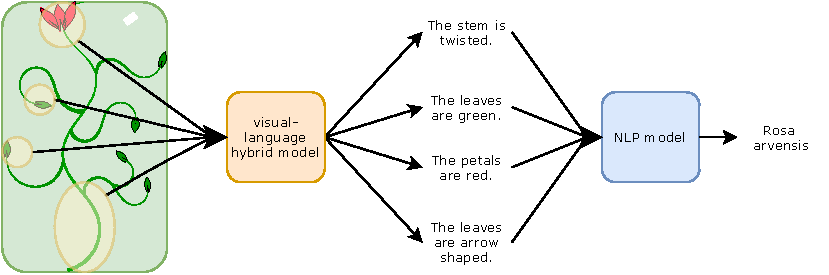
\includegraphics[width=\textwidth]{architecture.pdf}}
    \caption[Proposed architecture]{The proposed architecture by \textcite{ishikawa_contextual_2021} for species classification. The model input is an image. The first model will describe the attributes present in the image in natural language. The second model will take the output of the first model and will make a prediction. The intermediate results remain interpretable by using natural language.}
    \label{fig:intro}
\end{figure}

\textcite{ishikawa_contextual_2021} extended this bottleneck layer architecture by training a model that first learns the intermediate results.
The intermediate results are in this case similar to the semantic bottleneck.
The model is first trained to predict results in a for humans interpretable semantic way.
A second model will take these intermediate results to make a final prediction.
A more explainable, less rigid, model for species classification might be created by extending the concept of the semantic bottleneck layer from \textcite{ishikawa_contextual_2021} and splitting a regular convolution neural network (CNN) for image classification into two separate models that communicate using natural language.
The first model will describe species features and traits present in the image of a species, and the second model will take these descriptions and tries to infer the species (see Figure \ref{fig:intro}).
This way, DNNs reasoning for species classification can be tracked, mistakes can be spotted, and the models' performance can be improved.

The first model will be a visual-language model that extracts the species attributes from an image and describes its results in natural language. 
This vision hybrid model will be based on the researches of \textcite{radford_learning_2021} and \textcite{huang_interpretable_2020}.
Their findings allow the first model to learn to extract information from images by looking at raw text data that comes with image captions and describe objects present in those images.
This visual-language hybrid model will describe learned species attributes and use zero-shot learning to describe unseen (new) distinctive species traits.
By first describing traits, less abundant species can benefit from more abundant species if they share common traits.
This allows to model to perform better on long-tailed species datasets \autocite{van_horn_inaturalist_2018}.
Each species present in the dataset will be described equally well, because the DNN can learn traits from more abundant species.
The second model is a pure natural language processing (NLP) model that takes the partial descriptions and infer the species.
This way, a models reasoning for species predictions might be tracked by investigating the intermediate results \autocite{ishikawa_contextual_2021} and the final model results will be less rigid.

By first training the NLP model, we can create a model that can infer species based on partial textual descriptions of the species. 
As DNNs need we large datasets to properly learn the necessary features from the data \autocite{xue-wen_chen_big_2014, gheisari_survey_2017}, we first need to create this dataset.
This dataset needs as many unique descriptions as possible for each species, so for both a taxonomist and the NLP model, it would be possible to infer the species name based on provided descriptions.
We expect that a DNN model will learn the most important traits of a species if we can feed it enough unique descriptions.
For example, if the models sees multiple unique sentences about a European robin (also see \ref{fig:workflow}, the model will learn that an important trait for an European robin it its orange breast and plumage.
By applying posthoc explanatory techniques we can extract the most disciminative features from the text that are used for making a prediction.

This brings us to the first objective of this research: (1) creating an high-quality database with species and their descriptions.
We will train a model that can recognize descriptions sentences and deploy this model in a web crawler that can automatically query search engines.
The text from the returned URLs are broken down into single sentences and the text is classified by the model.
We hypothesise that this will result in a large database with clean descriptions about species, that an NLP model can learn distinctive features per species.

Once enough data is gathered, we train a NLP model to predict species based on the predictions.
The NLP model needs to make predictions on partial descriptions, but in the meantime, it should be clear which parts of the description data is used to make to prediction so the reasoning can be evaluated. 
This brings us to the second and third objective of this research: (2) creating an NLP model that can infer species names based on description data, (3) while in the meantime keeping traceability throughout the model.
This way we can validate if the model is focusing on useful traits of species.
We expect that if train an NLP model on text descriptions and extract the most important text for making a predictions, we can extract the most relevant and distinctive features of each species.

We first will describe our approach in the Methodology.
In Section \ref{par:dataset} we will describe how we gather enough description data per species.
In Sections \ref{par:Architecture} we define an NLP architecture and in Section \ref{par:keywords} we describe a method for comparing different posthoc explanatory techniques to extract the most distinctive traits of each species.
In Section \ref{par:results} we present the results and in Section \ref{par:discussion} we discuss our results.

\newpage
\section{Methodology} \label{par:methodoly}
\markboth{Approach}{Approach}
In Figure \ref{fig:workflow} a simplified version of the workflow can be found.
This chapter will give a detailed description of the steps.

\begin{figure} [htbp]
    \centering
    %\vspace{-2cm}
    \makebox[\textwidth][c]{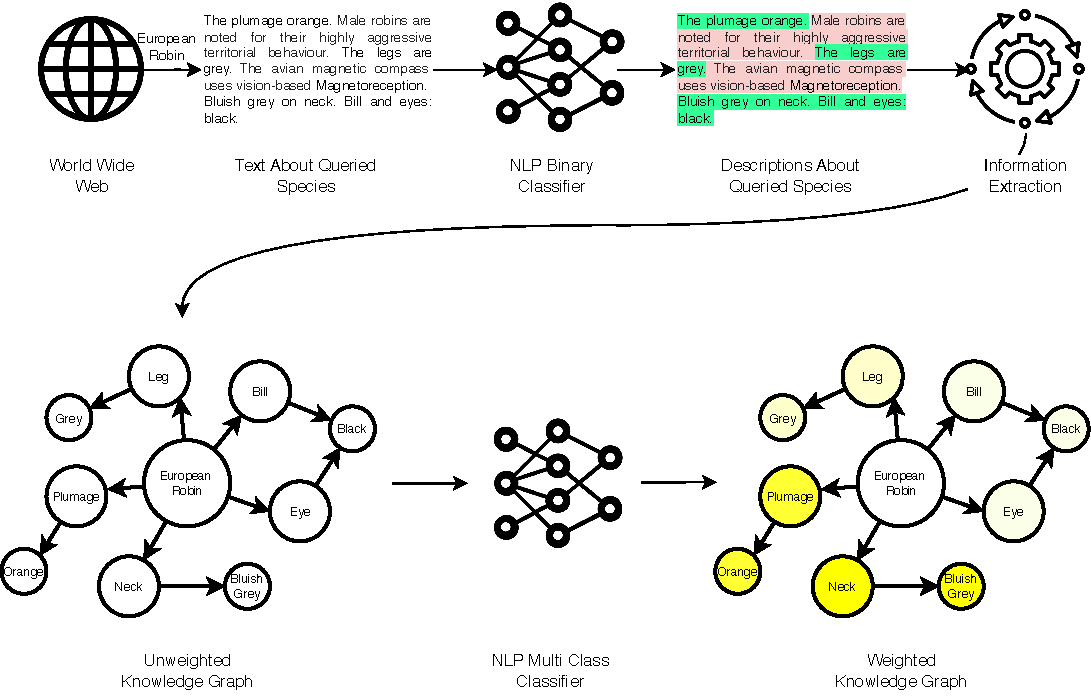
\includegraphics[width=\textwidth]{workflow.pdf}}
    \caption[Workflow]{A simplified workflow. Text data is used to train a model to recognize species description. In this case the paragraph titles are used as labels. The model is deployed in a web crawler that searches the web for species descriptions. These data are then used to train the NLP model independently of the visual-language hybrid model. The NLP model will focus on important words to recognise the species.}
    \label{fig:workflow}
\end{figure}

\subsection{Creating an Extensive Dataset} \label{par:dataset}
The World Wide Web also has potentially an endless amount of species descriptions available.
This makes the internet suitable for harvesting training data.
However, description sentences can be theoretically limitless, e.g. for a Brown Bear description text could be: "The fur is brown", "The brown bear has brown fur".
Sentences can have a more difficult semantic, e.g. "The fur of the Brown bear is similar to that of the Grizzly bear".
A classic machine learning approach that requires a rule-based match system for sentence classification is not possible. 
We first train a DNN that can classify text into description or non-description.
To properly train a deep learning model that can classify text data into description and non-description text, a large, accurate and consistent labelled dataset is needed \autocite{munappy_data_2019}.

\subsubsection{Training a Model for Text Classification}
%The internet has a vast amount of free data available that can be easily harvested.
We create this large dataset by scraping web pages from structured sources.
These sources (Wikipedia, Plant of the World Online (PoWO), Birds of the Word(BoW)), have a rich scholarly content about species.
These websites divide their information into paragraphs such as "Introduction", "Appearance", "Characteristics", "Habit".
These paragraph titles are used as labels and the text inside is used as training data.
In our case we stored text from paragraphs with titles like:  "Introduction" and "Habit" as negative labels and "Introduction" and "Appearance" as positive values, making this a two class classification problem. 
Random pages from Wikipedia that are not about species are also used to gather additional negative values.
We hypothesise that the model will be better in classifying text not related to species descriptions.
%BERT models use two specials tokens.
%This first token is always \verb|[CLS]|, which stands for "Classification".
%Using \verb|[CLS]|, the model knows the sequence is used for classification.
%The second token is \verb|[SEP]|, which stand for "Separation". 

However, this will not result in a consistent dataset.
Not all data will be labelled correctly as the paragraph titles are used as labels.
E.g. some species description might be located in the paragraph "Introduction" and some general information might be in the paragraph "Characteristics".
Consider the text "The European robin is red-breasted with distinctive eyes.".
This text is likely to be found in a paragraph about descriptions.
However, the text can also occur in the introduction paragraph about an European robin or it could be part of an image caption of an entirely different paragraph. 
In second cases the text will be miss classified with a binary cross entropy loss the model parameters will not be updated correctly. 
By implementing the semi-supervised loss function of \textcite{reed_training_2015}, this will be prevented to a certain extent.
Using natural language in combination with the soft loss function from \textcite{reed_training_2015}, allows the model for semi-supervised learning.
This combination has the advantage that it is now very easy to scale natural language training as we do not need annotated datasets.
If the predefined \(\beta\) reaches a threshold, the prediction is treated as correct and the loss is calculated accordingly.
\begin{equation} \label{eq:softloss}
 SoftLoss(q, t) = \sum_{k=1}^{L}[\beta t _k + (1- \beta )q _k]log(q _k)
\end{equation}
In equation \ref{eq:softloss}, \(q\) is directly used to calculate regression targets for each batch.
If the model prediction reaches the set threshold, the prediction is seen as a description label, but if the model prediction is below the threshold, the loss will be calculated accordingly.
In this thesis we use a \(\beta\) of 0.80. 

\subsubsection{Model Architecture} \label{par:Architecture}
As a base for the text classification model, we used a distilled version of the Bidirectional Encoder Representations from Transformers (BERT) \autocite{devlin_bert_2019}, called distilBERT \autocite{sanh_distilbert_2020}. 
This version is 60\% faster, has 40\% less parameters and still reaches 97\% on general language understanding \autocite{sanh_distilbert_2020}.
Using a pre-trained model can provide significantly improvements over models trained from scratch \autocite{mikolov_distributed_2013}.
The use of a pre-trained model is called transfer learning and could speed up the training process and increase the accuracy of the deep learning model.
Both distillBERT and BERT are already trained on a large corpus of English words and can be used freely.
\textcite{sun_how_2020} already investigated how to fine-tune BERT for text classification.
We use their findings on the full BERT model, to fine-tune the distilBERT model for description text classification.

Like \textcite{sun_how_2020} we first fit a fully connected linear layer with an input size of 768 and an output size of 512 on top of the BERT architecture. 
This linear layer is followed by a dropout layer (0.1) to enable some regularization.
The next fully connected linear layer has a input size of 512 and an output size of 2, as we are predicting two classes.
The final activation layer is a log-likelihood (log-softmax) activation function.
Using a log-softmax will slightly increase the error factor of the model over a normal softmax function, punishing mistakes a bit higher.
By taking the exponent, the standard likelihood (softmax) probabilities can be computed.

The basis distillBERT architecture can be fine-tuned further by updating the inner parameter of the transformer layers during training. 
This can be useful if BERT is utilised in the non-general domain \autocite{devlin_bert_2019, sun_how_2020, sanh_distilbert_2020}, which is the case with description data.
However, we decided not to fine-tune the inner workings of BERT for two reasons: 
(1) We used additional Wikipedia to increase the text data with negatives values.
These random Wikipedia pages are highly likely to contain information from the general
domain, resulting in a  data distribution close(r) to the general domain.
(2) A binary classification problem is a relatively simple task; updating the inner parameters during training cost additional time and computing power, while only resulting a small accuracy increase.

To prepare the text spans, we use the tokenizer of \textcite{wolf_huggingfaces_2020}.
The used BERT architecture can only process up to 512 token at once \autocite{sanh_distilbert_2020, devlin_bert_2019}.
Most tokenizers will truncate text spans larger then 512 tokens as most text information is in the beginning (head-encoding), end (tail-encoding) or beginning and end (head+tail-encoding).
We decide not truncated the text.
Instead we randomly split the text into text spans with a minimum of 10 words and a maximum of 512 words.
We hypothesised that the model might be better in recognising shorter description spans by splitting the raw spans.  
This way we enlarge the dataset, prevent loosing information with truncating spans larger then 512 tokens. 
We use a minimum of 10 words to prevent the model fixating on specific words.

The tokenizer of \textcite{wolf_huggingfaces_2020} returns a Python dictionary with the input ID's and the attention mask of the text.
E.g. by tokenizing the text "This is a test.", the tokenizer returns the following:
\verb|{'input_ids': [101, 2023, 2003, 1037, 3231, 1012, 102]|, 
\verb|'attention_mask': [1, 1, 1, 1, 1, 1, 1]}|.
\verb|[101]| indicates the start of a sequence and \verb|[102]| indicates the end of a sequence.
During the training the text is also padded to the maximum of 512 tokens and the attention masks are randomised between 0 and 1.

\subsubsection{Training \& Evaluation}
%We train the model on a Google Colab instance.
We use the Adam optimiser \autocite{kingma_adam_2017} during the training process.
The Adam optimiser has shown good performance when fine-tuning BERT for text classification \autocite{you_large_2020}.
The hyperparameters were set based on the paper of \textcite{sun_how_2020}.
The learning rate was set to 3e-5 and the batch size was set to 32.
During the training the gradients are clipped to prevent the gradients from becoming to large.
we train the model for 35 epochs.

As the dataset is will be unbalanced it will be evaluated with a precision-recall summary and a precision-recall curve.
The precision-recall summary and curves give more reliable results with an unbalanced dataset.
When the model reaches an f1-score of at least 0.9 on the testset, the model is tested on two additional left out databases, the \href{http://www.llifle.com/}{LLifle} dataset and the \href{https://www.worldagroforestry.org/}{AgroForestry} dataset.
If the model reaches a f1-score on 0.8 on these external datasets, the model will be deployed in a web crawler.
Before the text of the external dataset is tokenized, it is first cleaned of references and footnotes.
We no longer split the into random chunks, but we use a sentecizer of \textcite{honnibal_spacy_2020} to split the text into sentences.
This is also how random text will be treated that is gathered by the web crawler.
By splitting text into sentences instead of random text chunks we prevent information loss.

We again use the paragraphs as sample labels.
As the loss is no longer calculated, we simple calculate the prediction certainty of the model.
If the model reaches a certainty of 0.8 or higher (\(\beta\)) the prediction is treated as correct, in all other cases the predicted label is matches against the actual (paragraph) label.
This results in the following equation:
\begin{equation} \label{eq:softloss_ifthen}
(\hat{\gamma}^{(i)} >= \beta \rightarrow \hat{\gamma}^{(i)} = \gamma^{(i)}) \wedge ( \leftharpoondown \hat{\gamma}^{(i)} = \hat{\gamma}^{(i)})
\end{equation}
This is the loss function from \textcite{reed_training_2015}, only notated in an if-then statement to compensate for the miss labelled sentences of the external datasets.


\subsubsection{Gathering \& Storing Description Data}
We deploy the classification model in a web crawler.
This web crawler can automatically query search engines with a predefined list of birds and plants.
The list for plants is based on the \href{https://www.ipni.org/}{International Plant Name Index} (IPNI) and the list for birds is based on the database of \href{https://birdsoftheworld.org/bow/home}{Birds of the World} (BoW).
The IPNI database contains over 1,3 million plant species and the BoW database contains over ten thousand birds.
The IPNI database is large, containing all 1,3+ million known plant species.
There is a high chance that not all species in this database can be queried within the time-frame of this research.
Therefore we sort the plant species based on their number of description in the PoWO dataset that is used to train the classifier.
Plant species with a description have a higher chance of being described somewhere else on the web as the PoWO dataset is closely linked to the IPNI database.
This way we make sure that plant that will be queried have a high chance to contain a description somewhere on the web.
This is not an issue for the bird species; the BoW only contains 10k+ described birds.

The web crawler queries the search engines. 
This results in a list URLs with possible species descriptions.
We use five different ways of constructing a query: the name of the species without any additional search term and the name of the species plus description, diagnosis, attributes or captions.
We wrap quotations around the species to force the search engine to only return the exact species name. 
This way search engines cannot return any results that it deems similar.
Each query will return a list of candidate URLs and are appended to a list for a single species.
%The URL list is checked for duplicates as this is computationally less expense than calculating the cosine similarity for each sentence to drop duplicates.
The URLs are visited and all the text if retrieved.
If a URL points towards a PDF file er text file, it is skipped.
PDF files and text files are read line by line and not as a single text span and it is difficult to break these down into single sentences. 
Finally the header of the URL is checked against the queried species to make sure that the page really contains information about the queried species.
%Not every query will return correct websites, i.e. websites about the queried species.
%This way we prevent accidentally storing description data for the wrong species.

When the web page meets all criteria, the raw text is retrieved and broken down into single sentences. 
This makes sure the descriptions will be stored as much as possible per unique species trait.
The text is cleaned using several regular expressions. % LINK TO THE EXPRESSIONS
We use a pretrained sentecizer from \textcite{wolf_huggingfaces_2020} to split the text into single sentences.
Every sentence is checked against the train description classifier.
If a description is recognised by the model, the sentence is stored.
We use a threshold of 0.5 to determine if a sentence is a description or otherwise.
In Figure \ref{fig:webcrawler_sents} a small example can be found how the web crawler will process web pages and stores relevant information. 
Figure \ref{fig:webcrawler_sents_nopred} contains the original text before processing and in \ref{fig:webcrawler_sents_pred} the original text is processed into single sentences and each sentence is classified.

\begin{figure} [h!]
     \centering
     \begin{subfigure}[b]{1.00\textwidth}
         \centering
         %\hspace{-1.0cm}
         \frame{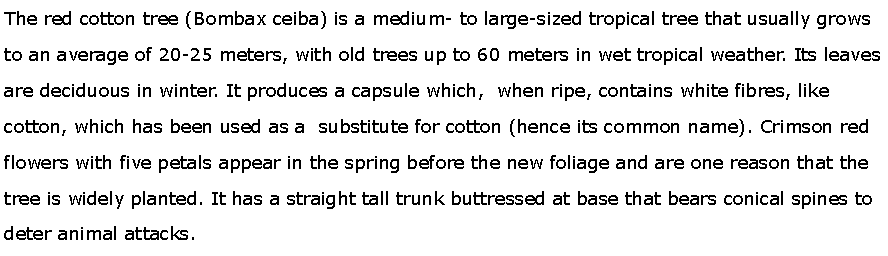
\includegraphics[width=\textwidth]{web_crawler_example_sents.pdf}}
         \caption[Raw text span example]{The raw text span from a web page. This a small portion of a web page about Bombax ceiba (source: \href{http://www.llifle.com/Encyclopedia/TREES/Family/Bombacaceae/31994/Bombax_ceiba}{Llilfe.com/Bomax\_ceiba}).}
         \label{fig:webcrawler_sents_nopred}
     \end{subfigure}
     \vfill
     \begin{subfigure}[b]{1.00\textwidth}
         \centering
         %\hspace{-0.5cm}
         \frame{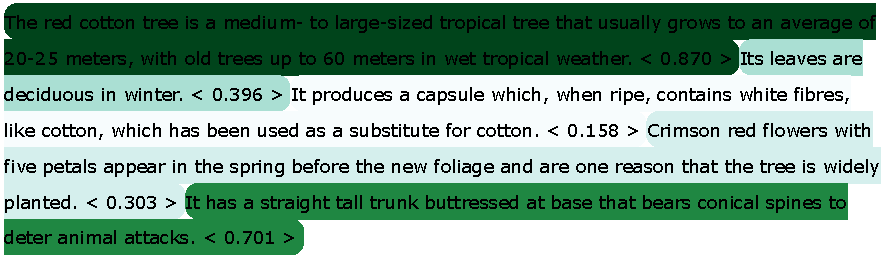
\includegraphics[width=\textwidth]{web_crawler_example_sents_preds.pdf}}
         \caption[Cleaned and classified text span example]{The cleaned and classified text. The text is coloured by the prediction value (high value is dark green, a low value near white). The prediction value of each sentence can be found at the end of the sentence.}
         \label{fig:webcrawler_sents_pred}
     \end{subfigure}
     \caption[Example of the web crawler process]{A small example how the web crawler processes and classifies data from a web page. The raw text span is cleaned from brackets, sources and other textual punctuation irregularities. After cleaning the text is split into single sentence. Each sentence is classified by the model. Sentences that reach or exceed the threshold of 0.5 are stored.}
     \label{fig:webcrawler_sents}
\end{figure}

Description sentences often name the species in the description, e.g. "Fagus sylvatica is a large tree, capable of reaching heights of up to 50 m (160 ft) tall." (source: \href{https://en.wikipedia.org/wiki/Fagus_sylvatica}{Wikipedia/wiki/Fagus\_sylvatica}).
Species names are replaced by the word "the species". 
In the example above in Figure \ref{fig:webcrawler_sents} the sentence is stored as: "The species is a large tree, capable of reaching heights of up to 50 m (160 ft) tall."
This way the NLP model will not have access to (parts of) the labels of the input data. In Figure \ref{fig:webcrawler_sents_nopred} and Figure \ref{fig:webcrawler_sents_pred} and example of a piece of text before and after processing can be found.

We deploy the web crawler for two weeks and the data that is gathered in these weeks is used in the next parts of this research. 

\begin{comment}
\subsubsection{Sentence Similarity}
There is a change that different web pages use the a common source for describing a species.
By checking for similar sentence within the same species we make sure the same sentence is not appended twice to the dataset and the train and test set are completely disjoint.
Like \textcite{reimers_sentence-bert_2019} we use the last hidden state of BERT (distilBERT in our case) and compute the cosine similarity to measure the distance between text spans.
Fortunately, this last hidden state is the output of a base BERT architecture.
However, the last hidden state output contain a matrix of 512 x 768. 
It is not feasibly to compute the cosine similarity distance for multiple matrices of this size.
By using a mean-pooling operation we create a vector of size 768 for every text span and compute the cosine distance for these text spans.
We first create a new dictionary that corresponds to the dictionary initialised by the tokenizer, \verb|{'input_ids': [], 'attention_mask': []}|.
We tokenize all the sentences we are comparing and append the tokens and masking to the correct key.
After all the sentences have been processed, we reformat the dictionary into a single tensor and push it trough the model.
This will result in a tensor of the number of sentences times 512 times 768. 
We sum the 3D matrix along the first axis, resulting in a 2D matrix.
The size of this matrix is the number of sentences time 768.
Each sentence is represented by a vector of size 768
Finally we calculate the cosine similarity between the sentences and drop sentences that exceed the threshold of 0.99.
In Figure \ref{fig:similarity_matrix} a comparison of a few fictional sentences can be found.
\begin{figure} [htbp]
    \centering
    \vspace{0cm}
    \hspace{-1cm}
    %\textbf{Similarity Matrix}
    \makebox[\textwidth][c]{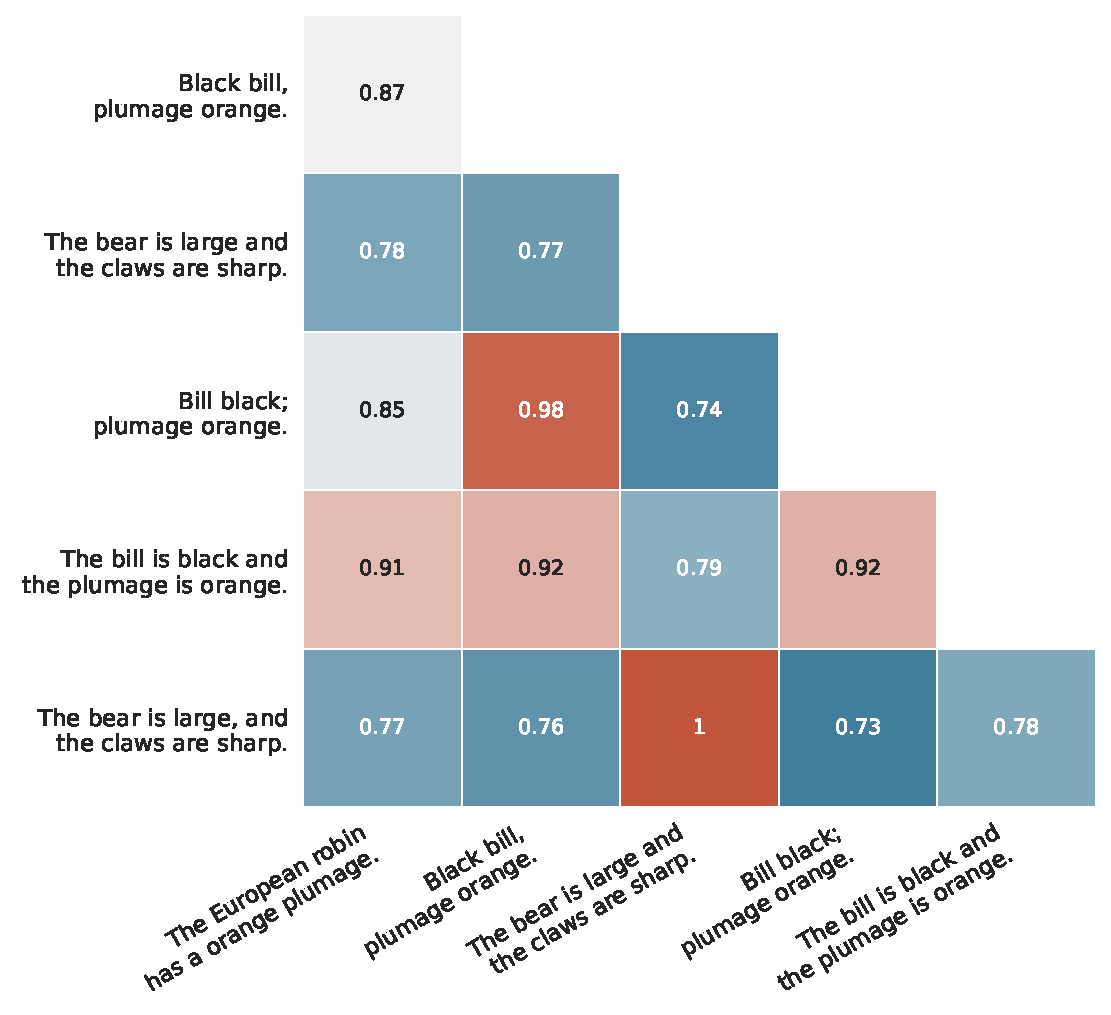
\includegraphics[width=0.7\textwidth]{similarity_matrix.pdf}}
    \caption[Example of sentence similarity]{An example for the calculation of sentence similarity. 
    %In this example the following sentences are compared.
     %0 - "The European robin has a orange plumage."
     %1 - "Black bill, plumage orange."
     %2 - "The bear is large and the claws are sharp."
     %3 - "Bill black; plumage orange."
     %4 - "The bill is black and the plumage is orange."
     %5 - "The bear is large, and the claws are sharp."
    In this case the sentences "Bill black; plumage orange." and "Black bill, plumage orange." reach a similarity score of 0.98. The word order and the punctuation is slightly different. In this case both sentences are stored in the database as it is highly likely they come from different sources. However in the case of "The bear is large and the claws are sharp." and "The bear is large, and the claws are sharp." the sentences are completely similar except for the punctuation. The sentences reach a similarity score of 1 (although this will be because of rounding). In the second case the sentences will come from a the same source and one of them will not be stored.}
    \label{fig:similarity_matrix}
\end{figure}

%Some databases store their description as one long sentence, describing multiple attributes in a single sentence e.g. "Leaves 5–9-foliolate; leaflets narrowly elliptic-obovate, entire, acuminate, 7–20 x 1.8–6.5 cm, glabrous; petiole 5.5 - 25 cm long, at the apex expanded into an almost circular disk." (source: \href{http://powo.science.kew.org/taxon/urn:lsid:ipni.org:names:1166232-2}{PoWO/Ceiba\_pentandra}). 
%This sentence is describing the leaves and the attributes in the same sentence. 

\subsubsection{Knowledge Graph}
A knowledge graph (KG) is a graph that contains interlinked descriptions, information has a formal structure that allows both people and computer to process the data unambiguously \autocite{petkova_crafting_2020}.
If we apply this to species descriptions we would expect the end up with a single graph per species, that contain descriptive information about that species in a semantic way.
These graphs can also be linked if species share common traits.
Creating a knowledge graph of the scraped data will results in a clean database.
This database will only contain subjects, relations and objects, also known as semantic triples. 
When feeding this data to the model it cannot be become dependent on artefacts such as word order, incorrect punctuation etc.


\begin{figure} [h!tb]
    \centering
    \begin{subfigure}[b]{1.0\textwidth}
        \centering
        %\vspace{0cm}
        \includesvg[inkscapelatex=false, width=\textwidth]{PoS_example.svg}
        \caption[Example of part of speech tagging (1)]{An example of part of speech and dependency parsing for the sentence "The Brown bear has brown fur.". The arrows contain the dependency tags and the words contain the part of speech tags.}
        \label{fig:PoS_example}
    \end{subfigure}
    \vfill
    \centering
    \begin{subfigure}[b]{1.0\textwidth}
        \centering
        %\vspace{0cm}
        \includesvg[inkscapelatex=false, width=\textwidth]{PoS_example2.svg}
        \caption[Example of part of speech tagging (2)]{An example of part of speech and dependency parsing for the sentence "The claws are sharp.". The arrows contain the dependency tags and the words contain the part of speech tags.}
        \label{fig:PoS_example2}
    \end{subfigure}
    \vfill
    \begin{subfigure}[b]{1.0\textwidth}
        \centering
        %\vspace{-2cm}
        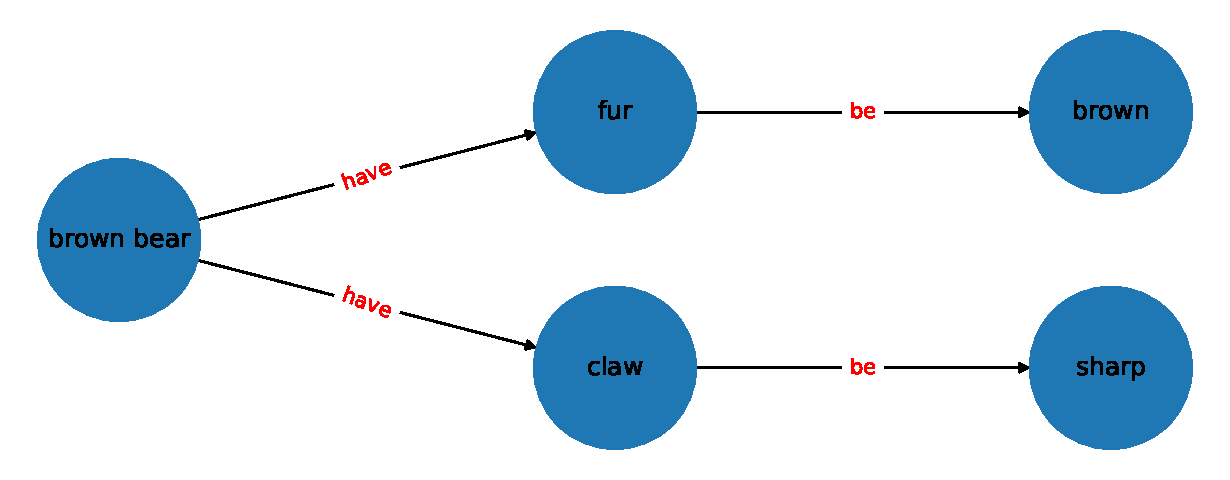
\includegraphics[width=\textwidth]{kn_example.pdf}
        \caption[Example of a knowledge graph]{The sentences result in five nodes (subject/object) and four edges (relations). The circles contain the objects/subjects and the arrows represent the relations.}
        \label{fig:graph_example}    
    \end{subfigure}
    \caption[Part of Speech tagging and knowledge graph]{The sentences are first broken down with the NLP pipeline of \textcite{honnibal_spacy_2020}. The extracted PoS tags and dependency tags are then used to construct the semantic triples In first case the first node is the normal subject (nsubj) combined witht the compound. The root verb of this subject is the relation and the direct object (dobj) of the verb is the object of the first semantic triple. For the last relation and node, the adjective modifier (amod) of the last node (fur) is used as object. In this case the relation is dependent on the PoS tag of the adjective modifier. In the last case the claws are a normal subject, but are treated as an object.}
    \label{fig:pos_pipeline}
\end{figure}
We use PoS tagging and dependency parsing to create a clean knowledge graph.
For PoS extracting we use the library of \textcite{honnibal_spacy_2020}.
This is a pretrained NLP model that can extract PoS tags and their dependencies.
We set up a rule-based system to extract data from the sentences.
In Figure \ref{fig:pos_pipeline} two example sentences can be found that are processed using PoS tagging and dependency parsing with the pretrained pipelines of \textcite{honnibal_spacy_2020}.
We have the benefit that we already know the broad subject of every sentence, which is the species.
Most researches do not have this and also need to determine the subject of every sentence \autocite{hutchison_knowledge_2013} like we do in \ref{fig:PoS_example}.
We know that every sentence describes the queries species, this means that we can have the species as starting node, even when the subject is not the species itself, see Figure \ref{fig:PoS_example2}.
By processing this in a rule-base system we create a knowledge graph like shown in Figure \ref{fig:graph_example}.
\end{comment}

\subsection{Inferring Species} \label{par:inferring}
For inferring species on partial descriptions we again use the distilled version of BERT \autocite{sanh_distilbert_2020, devlin_bert_2019} that we used for the binary classification of descriptions.
We simply replace the final linear layer of the model that currently has an output of two, with a linear layer that can output the number of species used in the training of the model.

We cannot split the data into a train and test set.
If we train-test split the data on species, during testing the model will be presented species it has never seen and it cannot predict the correct species.
An option would to train-test-spit the data so each species is represented in both the train and the test data.
However this brings the problem that we cannot asses if enough unique species traits are present in the train or the test data.


Finally, we extract the most relevant combination and present these chunks to 

To extract the most relevant we try different posthoc exploratory techniques and statistically assess which performs the best (also see Section \ref{par:keywords}).


\subsection{Retrieving Keywords} \label{par:keywords}
For retrieving key words from the description data we try several different posthoc explanation techniques. We implement all techniques with the Captum library from \textcite{kokhlikyan_captum_2020}.
\begin{itemize}
    \item Layer Integrated Gradients (LIG), based on the paper of \textcite{sundararajan_axiomatic_2017}. We use LIG with 20 steps and with 100 steps.
    \item Occlusions, based on \textcite{fleet_visualizing_2014}. Although this is originally used for explaining CNNs it can also be used to explain NLP models. We use two different version of occlusion, (1) with a window and stride of both 1. In this case each word will be replaced with a tensor of zeros to check the prediction changes of the model. (2) a window of 3\footnote{The windows is 1-dimensional in this case as the input vector is a tensor of the tokenised text.} and a stride of 2.
    \item Shapley Value Sampling (SVS) based on the papers of \textcite{castro_polynomial_2009, strumbelj_efficient_2010}. We use the Captum default of 25 samples.
    \item Layer Activation (LA), which simple computes the activation of the internal BERT embeddings for the inputs.
    \item Layer Gradient X Activation (LGXA), which is the element-wise multiplication of the gradients and the layers activation for a giver target with respect to the layer.
\end{itemize}

For comparing the techniques, we use the \href{http://www.vision.caltech.edu/visipedia/CUB-200-2011.html}{Caltech-UCSD Birds 200 dataset} (CUB-200) \autocite{welinder_caltech-ucsd_2010}.
The CUB-200 is a dataset with 200 bird species from Northern America.
Each bird is represented by approximately 60 images. 
Each of these images is hand annotated with traits that are present on the images.
We only use the text file with information if a certain trait is present on an image and concatenate this information for all the bird species.

We train a model on a subset on the BOW dataset, but we make sure all the CUB species are present in the training data.
The CUB birds are intersected with the BOW birds, this resulted in 94 common birds \footnote{The BOW dataset contains all described birds, some birds species have a different writing in the CUB data.}.
We random sample additional birds from the BOW dataset so the CUB birds make up about 5\% of the total data and resulting in 1,881 birds.
We do not split the model into train and test data, as evaluating with a test set has no use.
We use the same hyperparameters and architecture as we did for training the binary classification model (see \ref{par:Architecture}.
We only change the last linear output layer so it matches the number of species that are used during training.

We first match each text chunk against a bird glossary.
We use \href{https://en.wikipedia.org/wiki/Glossary_of_bird_terms}{W/Glossary/Birds} to construct this bird glossary list.
Each text chunk is matched against the bird glossary, if the chunk is a match we extract the most relevant words according to the aforementioned techniques.
The CUB-200 dataset is also matched against the bird glossary, so we can compare traits that are described in both datasets.
The most important word, together with the trait from the glossary is matched against the CUB-200 dataset to see which explanatory technique performs the best.
Text similarity with the CUB-200 dataset is used as a metric to compare the different techniques.
To compute the text similarity we use an untrained version of distillBERT and the cosine similarity.
For each bird, we select each trait of the text chunk and CUB dataset.
This will result in a list of text chunks for text chunks and for the CUB dataset.
We tokenize each chunk and push it trough the distilled version of BERT.
For each text chunk we sum the last hidden state along the first axis.
This will result in a matrix where the hidden state if summed for each token:
\begin{equation}
     \sum\nolimits_{j}^{} x_{ij} 
\end{equation}
Where~$i$ is 768 and~$j$ is the number of tokens. 
After this we simple compute the cosine similarity of each text chunk against all the text chunks of the CUB-200 dataset:
\begin{equation}
\cos ({\bf A},{\bf B})= {{\bf A} {\bf B} \over \|{\bf A}\| \|{\bf B}\|} = \frac{ \sum_{i=1}^{n}{{\bf A}_i{\bf B}_i} }{ \sqrt{\sum_{i=1}^{n}{({\bf A}_i)^2}} \sqrt{\sum_{i=1}^{n}{({\bf B}_i)^2}} }
\end{equation}
Where~$A$ is the vector of text chunk 1 and~$B$ the vector of text chunk 2.
Finally we statistically assess which of the exploratory techniques delivers the best performance.





\begin{comment}
We use the integrated gradients from \textcite{sundararajan_axiomatic_2017} to retrieve the most important keywords.
Integrated gradients are best used (1) to identify feature importance, in our case: which are the most important words used for a prediction and (2) to identify data skew, in our case this can be very important. %%% Add something about this.

Our code to calculate the integrated gradients is based on \textcite{gardner_allennlp_2017} and especially this  \href{https://github.com/allenai/allennlp/tree/master/allennlp/interpret}{this part} of their repository.
We use a zero input embedding as a baseline.
All irrelevant words will correspond to the baseline in this case.
We simply compute all the the gradients in a simple loop for a text span:
\begin{equation}
    x' +  \frac{\mathrm{k}}{\mathrm{m}} * (x - x')
\end{equation}
For this we use 20 steps to calculate the gradients as this is the minimum that \textcite{sundararajan_axiomatic_2017} found that could approximate the gradients by 5\%\footnote{The gradients are calculated from 0,00 to almost, but not exactly 1,00. As we are using 20 steps to calculate the gradients, we approximate the gradients by 5\% (\(\frac{1}{20} * 100 = 5\)). By increasing the number of steps, a better approximation of the gradients can be calculated. However, the computation time scales linearly with the number of steps.}.
We calculate the gradients for every input token and sum the gradients.
This leads to the following equation that approximates the gradients \autocite{sundararajan_axiomatic_2017}:
\begin{equation} \label{eq:integrad}
    {IntegratedGrads_i^{approx}} (x) ::= (x_i - x'_i) *  \sum\nolimits_{k=1}^{m}  \frac{\partial F(x' +  \frac{\mathrm{k}}{\mathrm{m}} * (x - x') }{\partial x_i} 
\end{equation}
\(i\) = feature (token/word)\newline
\(x\) = input (text span tokenized)\newline
\(x'\) = baseline (zero input embedding)\newline
\(k\) = scaled feature perturbation constant\newline
\(m\) = number of steps\newline
\((x - x')\) = difference from the baseline. \newline
\newline
By combining Equation \ref{eq:integrad} with PoS tagging and, we can extract the relevant PoS tags used for the prediction.
However, using a tokenizer can split certain words.
For example, for the sentence "The plant has 7 antheriferous stamens." we would expect nine token (beginning, words, point and ending).
Applying the BERT tokenizer on this sentence results in thirteen tokens:
%\newline
"\verb|[CLS] the plant has 7 ant ##her ##iferous st ##amen ##s. [SEP]|".
%\newline
if this happens we sum the gradients, because the sum of the gradients should equal 1.
In this example, both \verb|antheriferous| and \verb|stamens| will consist of three integrated gradients. 



\end{comment}


\newpage
\section{Results} \label{par:results}
\markboth{Results}{Results}
\subsection{Extensive dataset}
\subsubsection{Description Classification Model}

\begin{figure} [t]
    \centering
    \vspace{0cm}
    \makebox[\textwidth][c]{\includesvg[inkscapelatex=false, width=\textwidth]{histogram_text_length.svg}}
    \caption[Text length distribution for training web crawler model]{The result of scraping stuctured sources to train  a binary classification model for descriptions classification. The text length distribution before tokenization. The text spans are randomly split into chunks between 10 words and their length, with a maximum of 512 words to prevent truncation. Text spans with a length below 10 words are not split, resulting in some text lengths below 10. There are some text length with the maximum value of 512. This count is barely visible in the plot, so the x-axis limit is set to a max text length of 250.}
    \label{fig:text_length_distribution}
\end{figure}
Scraping the structured sources and using their paragraph titles resulted in 1,086,576 samples before splitting the sample into random text chunks.
%Each sample consists of a tuple, containing the label (0/1) and the text span.
Splitting the samples into text chunks resulted in 1,867,932 text chunks.
451,862 chunks have a label that corresponds to a description (label 1) and 1,416,070 chunks have a label that correspond to something different (label 0).
In Figure \ref{fig:text_length_distribution} the distribution after splitting the original samples in random chunks can be found.

The model is evaluated on a left out test set of 5\% and is evaluated on two left-out datasets, the \href{http://www.llifle.com/}{LLifle} dataset and the \href{https://www.worldagroforestry.org/}{AgroForestry} dataset
The summary performance metrics can be found in \ref{tab:precision_recall_metrics}.
The model reaches an high precision, recall and f1-score for both the "Non-Description" and "Description" class.
%These datasets are completely left out of the training/testing fase of the model.
%Together, these dataset contain 17,204 samples.
%771 text spans correspond to a description, and 16,433 text spans corresponds to something different.
%After the text has been cleaned and split into sentences there are 74,836 samples.
%There are 8,590 samples with a descriptions sentence and 66,246 samples that contain a sentence describing something %different.
%In Table \ref{tab:precision_recall_descriptionsmodel_external} the precision-recall summary for the external datasets can be found.
% Please add the following required packages to your document preamble:
% \usepackage{booktabs}
% Please add the following required packages to your document preamble:
% \usepackage{booktabs}
\begin{table}[ht]
\centering
\caption[Precision-recall metrics for the test dataset and the two left out datasets]{The precision-recall metrics for the binary classification model tested on the test dataset and two external datasets (LLifle and AgroForestry).}
\label{tab:precision_recall_metrics}
\begin{tabular}{@{}lcccccccc@{}}
\cmidrule(l){2-9}
 & \multicolumn{2}{c}{\textbf{Precision}} & \multicolumn{2}{c}{\textbf{Recall}} & \multicolumn{2}{c}{\textbf{f1-score}} & \multicolumn{2}{c}{\textbf{Support}} \\ \cmidrule(l){2-9} 
                 & Test & Extern & Test & Extern & Test & Extern & Test    & Extern \\ \midrule
                 & 0.98 & 0.99   & 0.99 & 0.98   & 0.99 & 0.98   & 167,955 & 66,051 \\
Description      & 0.97 & 0.83   & 0.95 & 0.90   & 0.96 & 0.86   & 57,864  & 8,785  \\ \midrule
Accuracy         &      &        &      &        & 0.98 & 0.97   & 225,819 & 74,836 \\
Macro Average    & 0.98 & 0.91   & 0.97 & 0.94   & 0.98 & 0.92   & 225,819 & 74,836 \\
Weighted Average & 0.98 & 0.97   & 0.98 & 0.97   & 0.98 & 0.97   & 225,819 & 74,836 \\ \bottomrule
\end{tabular}
\end{table}
As the the classes are imbalanced in both cases we also evaluated the model with a precision-recall plot.
The results of this plot can be found in Figure \ref{fig:precision-recall}.
\begin{figure} [h!]
     \centering
     \begin{subfigure}[b]{0.49\textwidth}
         \centering
         %\hspace{-0.5cm}
         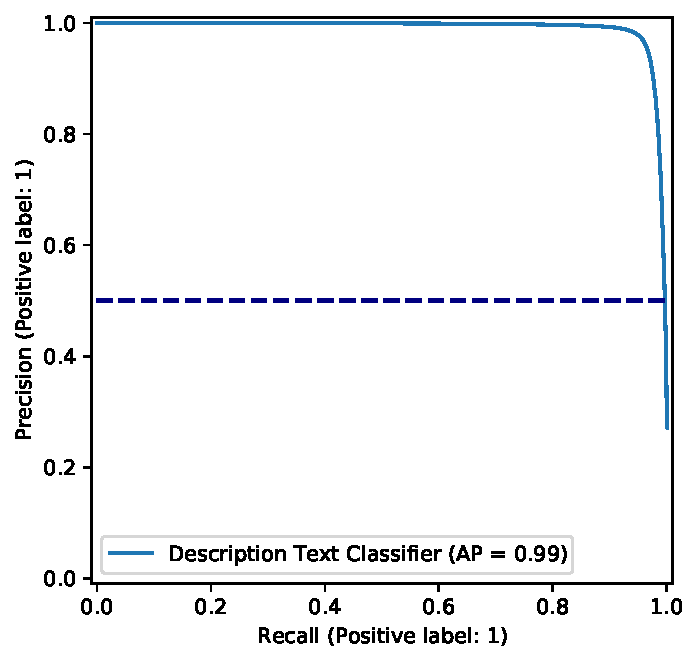
\includegraphics[width=\textwidth]{precision_recall_plot.pdf}
         \caption{The Precision-Recall curve for the test data.}
         \label{fig:precision_recall_curve_test}
     \end{subfigure}
     \hfill
     \begin{subfigure}[b]{0.49\textwidth}
         \centering
         %\hspace{-0.5cm}
         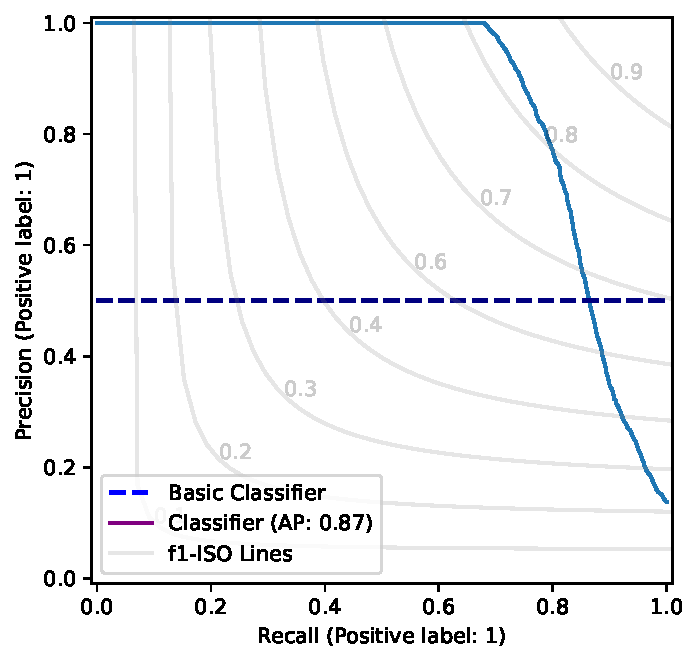
\includegraphics[width=\textwidth]{precision_recall_plot_extern.pdf}
         \caption{The Precision-Recall curve for the left out data.}
         \label{fig:precision_recall_curve_test_external}
     \end{subfigure}
     \caption[Precision recall curves for test and left-out datasets]{The precision-recall curve for the test dataset and the left out datasets. The model seems to perform reasonable in both cases. The the Average Precision (AP) reaches 99\% in the case of the test dataset and the AP reaches 96\% in the case of the left-out dataset. In both plots the blue dashed line indicates a baseline classifier.}
     \label{fig:precision-recall}
\end{figure}

\subsubsection{Dataset results}
\subsection{Key Words Inference}
\subsubsection{Similarity Results CUB}
\subsection{Species Classification}
\subsubsection{}
\section{Conclusion} \label{par:conclusion}
A binary description classification model can be trained by using structured webpages. 
By using the header as labels in combination with a semi-supervised loss, annotation can be prevented and the model can reach a high classification accuracy.

\section{Discussion} \label{par:discussion}
\subsubsection{Description Classifier}



\printbibliography
\end{document}